%% Author: Andrew J. Younge
%% PhD Thesis/Project

%$$$$$$$$$$$$$$$$$$$$$$$$$$$$$$$$$$$$$$$$$$$$$$$$$$$$$$$$$$$$$$$$$$$$%
\chapter{GPU-Passthrough Performance: A Comparison of KVM, Xen, VMWare ESXi, and LXC for CUDA and OpenCL Applications}
\label{chap:cloud2014}
%$$$$$$$$$$$$$$$$$$$$$$$$$$$$$$$$$$$$$$$$$$$$$$$$$$$$$$$$$$$$$$$$$$$$%


\begin{comment}
\begin{abstract}
As more scientific workloads are moved into the cloud, the need for high
performance accelerators increases.  Accelerators such as GPUs offer
improvements in both performance and power efficiency over traditional
multi-core processors; however, their use in the cloud has been limited.  Today,
several common hypervisors support GPU-passthrough, but their performance has
not been systematically characterized.  

In this chapter we show that low overhead PCI passthrough is achievable across 4
major hypervisors and two processor microarchitectures. We compare the performance of two generations of NVIDIA
GPUs within the Xen, VMWare ESXi, and KVM hypervisors, and we also compare the
performance to that of Linux Containers (LXC). We show that GPU passthrough to
KVM achieves 98--100\% of the base system's performance across two
architectures, while Xen and VMWare achieve 96--99\% of the base systems
performance, respectively.   In addition, we describe several
valuable lessons learned through our analysis and share the
advantages and disadvantages of each hypervisor/PCI passthrough solution. 

\end{abstract}
\end{comment}
\section{Introduction}
%Proposed contribution 
%\begin{enumerate} \item Demonstrate GPU Passthrough performance across 4
%standard hypervisors (what's the best word for this, given that LXC isn't
%really a hypervisor?) \item Any others?

%JP will write this, about ~ 3/4 of a page

%\end{enumerate}

% Add something that describes the necessity to use GPUs/Accellerators in "Cloud"

As scientific workloads continue to demand increasing performance at greater
power efficiency, high performance architectures have been driven towards heterogeneity and
specialization.  Intel's Xeon Phi, and GPUs from both NVIDIA and AMD represent some
of the most common accelerators, with each capable of delivering improved
performance and power efficiency over commodity multi-core CPUs. 


%Yet today's
%Infrastructure-as-a-Service (IaaS) clouds are largely homogeneous, with little
%or no access to accelerators.  


 Infrastructure-as-a-Service (IaaS) clouds have the potential to
democratize access to the latest, fastest, and most powerful computational
accelerators.  This is true of both public and private clouds.  Yet today's
clouds are typically homogeneous without access to even the most commonly used
accelerators.  Historically, enabling virtual machine access to GPUs and other PCIe devices has
proven complex and error-prone, with only a small subset of GPUs being
certified for use within a few commercial hypervisors.  This is especially true
for NVIDIA GPUs, likely the most popular for scientific computing, but whose
drivers have always been closed source.  

Given the complexity surrounding the choice of GPUs, host systems, and
hypervisors, it is perhaps no surprise that Amazon is the only major cloud
provider offering customers access to GPU-enabled instances.  All of this is
starting to change, however, as open source and other freely available
hypervisors now provide sufficiently robust PCI passthrough functionality to
enable GPU and other accelerator access whether in the public or private cloud.

Today, it is possible to access GPUs at high performance within all of
the major hypervisors, merging many of the advantages of cloud computing (e.g. custom
images, software defined networking, etc.)  with
the accessibility of on-demand accelerator hardware.  Yet, no study to date has
systematically compared the performance of PCI passthrough across all major
cloud hypervisors.  Instead, alternative solutions have been proposed that
attempt to virtualize the GPU~\cite{Duato2010rc}
, but sacrifice performance.

%Instead, alternative solutions have been proposed that attempt to virtualize the
%GPU~\cite{Duato2010rcuda, shi2012vcuda, Gupta:2009, giunta2010gvirtus}. These solutions, typically based on library
%interposition, essentially redirect the CUDA, OpenCL, OpenGL, or DirectX library calls in order
%to access GPUs via a network or other shared memory device.  This approach works
%well for some workloads, including desktop virtualization, but is insufficient for performance
%critical code.  

In this chapter, we characterize the performance of both NVIDIA Fermi and Kepler GPUs
operating in PCI passthrough mode in VMWare VSphere, Linux KVM, Xen, and Linux
Containers (LXC).  Through a series of microbenchmarks as well as scientific and
Big Data applications, we make two contributions: 

\begin{enumerate}
\item We demonstrate that PCI passthrough at high performance is possible for
GPUs across 4 major hypervisors.
\item We describe the lessons learned through our performance analysis, as well as the relative advantages
and disadvantages of each hypervisor for GPU support.
\end{enumerate}

%In this paper we characterize the performance of the NVIDIA Kepler K20 GPU
%across VMWare VSphere 5.5, KVM, Xen, and Linux Containers (LXC).  Through a
%series of microbenchmarks as well as common scientific and Big Data
%applications, we make the following contributions: 

%\begin{enumerate} 

%\item[1.] Demonstrate GPU passthrough performance across 4 major hypervisors.  

%\item[2.] Describe the lessons learned through our PCI passthrough hypervisor
%analysis.

%\end{enumerate}

%The remainder of this paper is organized as follows: in
%Section~\ref{BACKGROUND}, we describe PCI passthrough within the context of
%%both GPUs and general PCI devices; in Section~\ref{RELATED}, we describe the
%prior work in the area of virtual machine access to GPUs; in
%Section~\ref{METHOD} we present our experimental methodology, benchmarks, and
%system characteristics; in Section~\ref{RESULTS} we characterize each
%hypervisor using both microbenchmarks and real applications; in
%Section~\ref{ANALYSIS} we analyze and discuss the results; 


%\section{Background}\label{BACKGROUND}
%about 1 page.  JP will coordinate, may get some background from Andrew.

\begin{comment}
\subsection{PCI Passthrough}

Input/Output Memory Management Units, or IOMMUs, play a fundamental roll in the PCI-Passthrough virtualization mechanism. Like traditional MMUs that provide a virtual memory address space to CPUs \cite{Jacob1998}, an IOMMU serves the fundamental purpose of connecting a direct memory access (DMA) capable I/O bus to main memory. The IOMMU unit, typically within the chipset, maps device virtual addresses to physical memory addresses. This process also has the added improvement of guaranteeing device isolation by blocking rouge DMA and interrupt requests \cite{yassour2008direct}, with a slight overhead, especially in early implementations \cite{ben2007price}. 

The IOMMU is usually used for providing high performance networking solutions to guest VMs \cite{rixner2008network, dong2008sr, liu2010ipdps} it is also a key component for enabling GPU PCI-Passthrough. As most hypervisors remap guest main memory, and current graphics cards use DMA to read and write between main memory and GPU device memory. Without IOMMU, the PCI device's bus wouldn't be useable within a guest VM. With IOMMU,  DMA remapped is utilized for a given virtual address space within a guest VM, thereby allowing for the PCI device to be used directly within the guest. This also eliminates the need for any resource-intensive emulation or other host involvement after the guest VM is created.

Currently two major IOMMU implementations exist, VT-d \cite{hiremane2007intel, intelvtd} and AMD-Vi\cite{amd2007technology} by Intel and AMD, respecively. Both specifications provide DMA remapping to enable PCI-Passthrough as well as other features such as Interrupt remapping, hypervisor snooping, and security control mechanisms to esnure proper and efficient hardware utilization.  While other IOMMU implementations exist, this manuscript focuses exclusively on VT-d due to our use of two different Intel architectures.  


% I don't think there's much advantage to introducing SR-IOV here as these devices are not using it and its out of the scope

\subsection{GPU Passthrough}

While generic PCI-Passthrough can be used with IOMMU technologies to pass through various PCI-Express devices, GPUs represent a special case which has hampered usage until only recently. In traditional usage, GPUs usually serve as VGA devices primarily to render screen output and while the purposes of scientific computing using GPUs do not require this function, it still exists in legacy. In GPU-Passthrough, another VGA device (such as onboard graphics built into the motherboard) is necessary to serve as the primary display for the host, as well as providing emulated VGA devices for each guest VM. Most GPUs also have a video bios that requires full inititialization and reset functions, which is often difficult due to the proprietary nature of the cards and their drivers. 

There is a wide range of implementation differences of PCI-Passthrough between the hypervisors studies in this manuscript. However, type 1 and 2 hypervisors such as KVM, Xen, and VMWare all operate on similar principals. LXC, a linux container solution, does not use traditional PCI-Passthrough of GPUs, as described later.  For hypervisors, the IOMMU must first be built into the kernel and enabled within the kernel bootloader parameters. This allows DMA and interrupt mechanisms to be properly initialized before any devices are initialized. Next, the original device's drivers must be blacklisted, either within the kernel or directly as a module to ensure the PCI device (in our case the GPU) is not initialized by the host. Later in the boot order, a hypervisor specific module will sieze the device to prevent any furter initialization or tampering, while also making the device visible to the host. In KVM, this is accomplished with the new vgio driver to seize a GPU whenb booting. Xen uses the pci-back driver and VMWare leverages their VMDirectPath I/O mechanism for similar results. During guest VM creation, the hypervisor will relinquish control of the PCI device and the device will be passed through to the guest. Finally, the VM can load standard drivers and use the device as expected, in our case for scientific computing problems.


\end{comment}



\section{Related Work \& Background}\label{RELATED}

GPU virtualization and GPU-passthrough are used within a variety of contexts,
from high performance computing to virtual desktop infrastructure.  Accessing one or
more GPUs within a virtual machine is typically accomplished by one of two
strategies: 1) via API remoting with device emulation; or 2) using PCI
passthrough.  


\subsection {GPU API Remoting}

rCUDA, vCUDA, GViM, and gVirtuS are well-known API
remoting solutions%~\cite{Duato2010rcuda, shi2012vcuda, Gupta:2009, giunta2010gvirtus}.
Fundamentally, these approaches operate similarly by splitting the driver into a
front-end/back-end model, where calls into the interposed CUDA library
(front-end)  are sent via shared memory or a network interface to the back-end
service that executes the CUDA call on behalf of the virtual machine.  Notably,
this technique is not limited to CUDA, but can be used to decouple OpenCL,
OpenGL, and other APIs from their local GPU or accelerator. 

%The general purpose of GPU virtualization is to centralize management and administration by utilizing overall hardware resources and improving scalability~\cite{Yang2012}. We can categorize virtualization into  two types according to the defined virtualization boundary between the stack and physical GPU hardware. One is to run the graphics driver in the host/hypervisor such as API Remoting and device emulation, and the other is to run the graphic driver stack inside the Virtual Machine (VM) such as pass-through technique~\cite{Dowty2009, Yang:2012}.

%NVIDIA's Compute Unified Device Architecture (CUDA) is a parallel computing platform and scalable parallel programming model~\cite{Yang2012, Yang:2012, Song:2013}. For the virtualization of the CUDA Runtime API for VMs, several virtualization approaches are available, such as rCUDA, vCUDA, GPU-accelerated Virtual Machines(GViM) and gVirtuS~\cite{Yang:2012, Gupta:2009}. rCUDA employs Sockets API to let the client and server have communication with each other. As a General Purpose Graphics Processing Unit (GPGPU) computing solution, vCUDA lets applications in VMs access graphics hardware. GViM virtualizes the graphics accelerator at the level of abstraction, leverages the CUDA APIs and their open source counterparts, and offers low overheads and direct access to accelerator resources by guest OS. gVirtuS is an hypervisor-independent GPU Virtualization Service. Also, as a new approach to GPU resource management, Gdev integrates runtime support into the OS by adopting more appropriate scheduling algorithm for compute-intensive workload~\cite{Kato:2012}. 

The performance of API-remoting depends largely on the application and the
remoting solution's implentation.  Bandwidth
and latency-sensitive benchmarks and applications will tend to expose performance bottlenecks
more than compute-intensive applications.  Moreover, solutions
that rely on high speed networks, such as Infiniband, will compete with
application-level networking for bandwidth.  


\subsection{PCI Passthrough}

Input/Output Memory Management Units, or IOMMUs, play a fundamental roll in the
PCI-passthrough virtualization mechanism. Like traditional MMUs that provide a
virtual memory address space to CPUs \cite{Jacob1998}, an IOMMU serves the
fundamental purpose of connecting a direct memory access (DMA) capable I/O bus
to main memory. The IOMMU unit, typically within the chipset, maps device
virtual addresses to physical memory addresses. This process also has the added
improvement of guaranteeing device isolation by blocking rogue DMA and interrupt requests \cite{yassour2008direct}, with a slight overhead, especially in early implementations \cite{ben2007price}. 

%The IOMMU is usually used for providing high performance networking solutions
%to guest VMs \cite{rixner2008network, dong2008sr, liu2010ipdps} it is also a
%key component for enabling GPU PCI-passthrough. As most hypervisors remap guest main memory, and current graphics cards use DMA to read and write between main memory and GPU device memory. Without IOMMU, the PCI device's bus wouldn't be useable within a guest VM. With IOMMU,  DMA remapped is utilized for a given virtual address space within a guest VM, thereby allowing for the PCI device to be used directly within the guest. This also eliminates the need for any resource-intensive emulation or other host involvement after the guest VM is created.

Currently two major IOMMU implementations exist, \mbox{VT-d}  and
{AMD-Vi} by Intel and AMD, respectively. Both
specifications provide DMA remapping to enable PCI-passthrough as well as other
features such as interrupt remapping, hypervisor snooping, and security control
mechanisms to ensure proper and efficient hardware utilization. PCI passthrough has been studied within the context of networking~\cite{liu2010ipdps}, storage~\cite{jujjuri2010virtfs}, and other PCI-attached devices; however, GPUs have historically lagged behind other devices in their support for virtual
machine passthrough.  


% I don't think there's much advantage to introducing SR-IOV here as these devices are not using it and its out of the scope

\subsection{GPU Passthrough, a Special Case of PCI Passthrough}

While generic PCI passthrough can be used with IOMMU technologies to pass
through many PCI-Express devices, GPUs represent a special case of PCI
devices, and a special case of PCI passthrough. In traditional usage, GPUs usually serve as VGA devices primarily to
render screen output, and while the GPUs used in this study do not render screen
out, the function still exists in legacy. In GPU-passthrough, another VGA device
(such as onboard graphics built into the motherboard, or a baseboard management
controller) is necessary to serve as the primary display for the host, as well
as providing emulated VGA devices for each guest VM. Most GPUs also have a video
BIOS that requires full initialization and reset functions, which is often difficult due to the proprietary nature of the cards and their drivers. 

%There is a wide range of implementation differences of PCI-passthrough between
%the hypervisors studies in this manuscript. However, type 1 and 2 hypervisors
%such as KVM, Xen, and VMWare all operate on similar principals. LXC, a linux
%container solution, does not use traditional PCI-passthrough of GPUs, as described later.  For hypervisors, the IOMMU must first be built into the kernel and enabled within the kernel bootloader parameters. This allows DMA and interrupt mechanisms to be properly initialized before any devices are initialized. Next, the original device's drivers must be blacklisted, either within the kernel or directly as a module to ensure the PCI device (in our case the GPU) is not initialized by the host. Later in the boot order, a hypervisor specific module will sieze the device to prevent any furter initialization or tampering, while also making the device visible to the host. In KVM, this is accomplished with the new vgio driver to seize a GPU whenb booting. Xen uses the pci-back driver and VMWare leverages their VMDirectPath I/O mechanism for similar results. During guest VM creation, the hypervisor will relinquish control of the PCI device and the device will be passed through to the guest. Finally, the VM can load standard drivers and use the device as expected, in our case for scientific computing problems.


Nevertheless, for applications that require native or near-native GPU performance across the
full spectrum of applications with immediate access to the latest GPU drivers
and compilers, GPU passthrough solutions are preferrable to API remoting.  Today, Citrix Xenserver, open source Xen \cite{Yang:2012}, and VMWare ESXi ~\cite{Dowty2009}, and most recently KVM all support GPU passthrough.  To our knowledge, no one has systematically characterized the performance of GPU passthrough across a range of hypervisors, across such a breadth of benchmarks, and across multiple GPU generations as we do.  

%To our knowledge, this work is the first that describes the use of NVIDIA Tesla GPUs specifically with the KVM hypervisor. % as vfio functionality necessary was only recently introduced in the 3.9 Linux kernel. 



%To cope with I/O performance degradation, Virtual Machine Monitor (VMM)-bypass I/O technologies, including PCI passthrough and SR-IOV, have been introduced~\cite{Nakada:2012}. Device pass-through allows guest operating system to have exclusive access~\cite{Yang:2012}. PCI Express (PCIe) Single-root I/O Virtualization (SR-IOV) works by assigning directly hardware resource of I/O devices to a VM to reduce I/O performance degradation~\cite{Suzuki:2010}. To make migration and checkpoint/restart possible over VMM-bypass I/O devices, Symbiotic Virtualization (SymVirt) is proposed, without the virtualization overhead during normal operations~\cite{Nakada:2012}. And GPUDirect RDMA (GDR) is a feature introduced in CUDA with collaboration of NVIDIA and Mellanox for InifiniBand clusters, that allows third party devices like network adapters to directly access data in GPU device memory, over the PCIe bus~\cite{Potluri:2013}.

%The performance of a virtualized GPU depends on the characteristics of the application under test~\cite{Dowty2009}. API Remoting or device emulation causes significant performance degradation relative to native hardware. But, device pass-through technique can achieve near-native performance and GPU feature set, and maintain driver easily~\cite{Yang:2012}. The inner communication in VM is not through the real hardware but just in the memory on the real machine~\cite{Yang2012}. Also, power-performance efficiency model is proposed at exascale by identifying bottlenecks of power-performance and their main causes on GPU-based heterogeneous HPC systems~\cite{Song:2013}.


\section{Experimental Methodology}\label{METHOD}
%In this paper, we are comparing the performance of a standard CentOS 6.4 virtual
%against a comparable CentOS 6.4 bare metal machine.  However, each hypervisor
%has its own system requirements which


\subsection{Host and Hypervisor Configuration}

We used two hardware systems, named Bespin and Delta, to evaluate four
hypervisors.
The Bespin system at USC/ISI represents Intel's Sandy Bridge microarchitecture with a Kepler class K20 GPU. The Delta system, provided by the FutureGrid project \cite{www-futuregrid}, represents the Westmere microarchitecture with a Fermi class C2075 GPU. 
%  Bespin and Delta are representative of
%Intel's Sandy Bridge and Westmere microarchitectures, respectively.  The Bespin
%system includes a Kepler class K20 GPU, while the Delta system includes a Fermi
%class C2075 GPU.  The Delta system was available as part of the FutureGrid project
Table~\ref{HOSTS} provides
the major hardware characteristics of both systems.  Note that in addition, both
systems include 10 gigabit Ethernet, gigabit Ethernet, and either FDR or QDR
Infiniband. Our experiments do not emphasize networking, and we use the gigabit
ethernet network for management only.


\begin{table}
\small
\renewcommand{\arraystretch}{1.3}
\caption{Host hardware configurations}
\label{HOSTS}
\centering
\begin{tabular}{|l||l|l|}
\hline
 & Bespin & Delta  \\ \hline
CPU (cores)  & 2x E5-2670 (16)  & 2x X5660 (12) \\ \hline
Clock Speed & 2.6 GHz & 2.6 GHz \\ \hline 
RAM &  48 GB &  192 GB \\ \hline
NUMA Nodes & 2 & 2 \\ \hline
GPU &  1x K20m &  2x C2075 \\ \hline

\end{tabular}
\end{table}

A major design goal of these experiments was to reduce or eliminate NUMA effects
(non-uniform memory access) on the PCI passthrough results in order to
facilitate fair comparisons across hypervisors and to reduce experimental noise.  To this end, we
configured our virtual machines and containers to execute only on the NUMA node
containing the GPU under test.  We acknowledge that the NUMA effects on
virtualization may be interesting in their own right, but they are not the
subject of this set of experiments.

We use Bespin and Delta to evaluate three hypervisors and one container-based
approach to GPU passthrough. The hypervisors and container system, VMWare ESXi,
Xen, KVM, and LXC, are summarized in Table~\ref{HYPERVISORS}.  Note that each
virtualization solution imposes its own unique requirements on the base
operating system.  Hence, Xen's Linux kernel refers to the Domain-0 kernel,
whereas KVM's Linux kernel represents the actual running kernel hosting the KVM
hypervisor.  Linux Containers share a single kernel between the host
and guests, and VMWare ESXi does not rely on a Linux kernel at all.  

Similarly, hypervisor requirements prevented us from standardizing on a single host operating system.  For Xen
and KVM, we relied on the Arch Linux 2013.10.01 distribution because it provides
easy access to the mainline Linux kernel.  For our LXC tests, we use CentOS
6.4 because its shared kernel was identical to the base CentOS 6.4 kernel used
in our testing.  VMWare has a
proprietary software stack.  All of this makes comparison challenging, but as we describe in
Section~\ref{GUESTS}, we are running a common virtual machine across all
experiments.

%Our base host system is composed of 2x 8-core Intel Xeon E5-2670 CPUs and 48
%GB of RAM split into two NUMA nodes of one CPU socket and 24 GB RAM.  A single
%NVIDIA Kepler K20m GPU available, and is attached to NUMA node 0.  In addition,
%the node is equipped with 10 Gb Ethernet, FDR Infniband, and gigabit Ethernet.
%All benchmarking is contained within a single node, so neither the 10 Gb
%Ethernet adapter or the FDR Infiniband adapter were used.  The gigabit Ethernet
%adapter was used only as a management network for guest access.

%For our experiments, we compare VMWare ESXi 5.5.0, KVM from Linux Kernel 3.12
%with QEMU version 1.7, Xen 4.3.0 with Linux kernel 3.12 Dom0, and LXC containers based on
%2.6.32-358.23.2 from CentOS 6.4   Both KVM and Xen use an Arch Linux 2013.10.01
%installation as their base distribution.  VMWare ESXi is a proprietary
%bare-metal software stack and is not based on Linux.


%In Table~\ref{HYPERVISORS} we describe the system configuration for each
%hypervisor.  Note that the column Linux Kernel describes the

\begin{table}
\small
\renewcommand{\arraystretch}{1.3}
\caption{Host Hypervisor/Container Configuration}
\label{HYPERVISORS}
\centering
\begin{tabular}{|l||l|l|}
\hline
Hypervisor & Linux Kernel & Linux Version \\ \hline 
KVM & 3.12 & Arch 2013.10.01 \\ \hline 
Xen 4.3.0-7 & 3.12 & Arch 2013.10.01 \\ \hline
VMWare ESXi 5.5.0 & N/A & N/A \\ \hline
LXC & 2.6.32-358.23.2 & CentOS 6.4 \\ \hline

\end{tabular}
\end{table}


%We treat each hypervisor as its own system, comparing a VM composed of CentOS
%6.4 with a bare metal machine running CentOS 6.4. This results in challenges
%when comparing one hypervisor to another 



\subsection{Guest Configuration}\label{GUESTS}

We treat each hypervisor as its own system, and compare virtual machine guests
to a base CentOS 6.4 system. The base system and the guests are all composed of
CentOS 6.4 installation with a 2.6.32-358.23.2 stock
kernel and CUDA version 5.5. Each guest is allocated 20 GB of RAM and a full CPU
socket (either 6 or 8 CPU cores).  Bespin experiments received 8 cores and Delta
experiments received 6 cores.  VMs were restricted to a single NUMA node.  On
the Bespin system, the K20m GPU was attached to NUMA node 0.  On the Delta
system, the C2075 GPU was attached to NUMA node 1.  Hence VMs ran on NUMA node 0
for the Bespin experiments, and node 1 for the Delta experiments. 



\subsection{Microbenchmarks}

Our experiments are composed of a mix of microbenchmarks and application-level
benchmarks, as well as a combination of CUDA and OpenCL benchmarks.  The SHOC
benchmark suite provides a series of microbenchmarks in both OpenCL and
CUDA~\cite{Danalis:2010}. For this analysis, we focus on the OpenCL benchmarks
in order to exercise multiple programming models.  Benchmarks range from
low-level peak Flops and bandwidth measurements, to kernels and
mini-applications.  


\subsection{Application Benchmarks}
For our application benchmarks, we have chosen the LAMMPS molecular
dynamics simulator~\cite{LAMMPS}, the GPU-LIBSVM~\cite{Athanasopoulos:2011}, and the
LULESH shock hydrodynamics simulator~\cite{LULESH}.  These represent a range of
computational characteristics, from computational physics to big data analytics, and are
representative of GPU-accelerated applications in common use. 

\paragraph {LAMMPS} The Large-scale Atomic/Molecular Parallel Simulator
(LAMMPS), is a parallel molecular
dynamics simulator~\cite{LAMMPS,Plimpton1995} used for production MD simulation
on both CPUs and GPUs~\cite{LAMMPSGPU}.  LAMMPS has two packages for GPU
support, the USER-CUDA and GPU packages.
With the USER-CUDA package, each GPU is used by a single CPU, whereas the GPU
package allows multiple CPUs to take advantage of a single GPU.  There are
performance trade-offs with both approaches, but we chose to use the GPU package
in order to stress the virtual machine by exercising multiple CPUs.  Consistent
with the existing GPU benchmarking approaches, our results are based on the
Rhodopsin protein.

%Atomic LJ fluid has low arithmetic intensity, and small neighbor list. As a result, it shows modest speedup of LAMMPS performance improvements using GPU.
%Gay-Berne has high arithmetic intensity and pairwise force calculation. As a result, it shows upper side of LAMMPS performance improvements using GPU.
%In the case of Rhodopsin, Poisson solver running on CPU takes large percentage of the total time, and shows least speedup using GPU among the three benchmarks.
%We believe that those three benchmarks cover a reasonable range of the characteristis of production applications using both CPU cores and a GPU.
%And our study of virtualization overhead of those benchmarks can give the glimpse of the overehad of virtualization of production applications. 

\paragraph{GPU-LIBSVM} LIBSVM is a popular implementation~\cite{Chang:2011} of
the machine learning classification algorithm support vector machine
(SVM). GPU-accelerated LIBSVM~\cite{Athanasopoulos:2011} enhances LIBSVM by
providing GPU-implementations of the kernel matrix computation portion of the
SVM algorithm for radial basis kernels. For benchmarking purposes we use the
NIPS 2003 feature extraction gisette data set. This data set has a high
dimensional feature space and large number of training instances, and these
qualities are known to be computational intensive to generate SVM models. The
GPU-accelerated SVM implementation shows dramatic improvement over the CPU-only
implementation.


\paragraph{LULESH} Hydrodynamics is widely used to model continuum properties
and interactions in materials when there is an applied
force~\cite{LLNL-TR-490254}. Hydrodynamics applications consume approximately one third
of the runtime of data center resource throughout the U.S. DoD (Department of
Defense). The Livermore Unstructured Lagrange Explicit Shock Hydro (LULESH) was
developed by Lawrence Livermore National Lab as one of five challenge problems in the DARPA UHPC program.
LULESH is widely used as a proxy application in the U.S. DOE (Department of
Energy)  co-design effort for exascale applications~\cite{LULESH}. 


%LULESH 1.0
%includes both Kepler and Fermi GPU models which we use in our benchmarking. 
 

\section{Performance Results}\label{RESULTS}

%note: to keep the table readable in plaintext, be sure to set your textwidth=300 (or so), so that lines don't wrap and get ugly.  This has no effect on the Latex output.
\begin{table*}
%\rowcolors{2}{gray!25}{white}
\footnotesize
\caption{SHOC overheads for Bespin (K20) expressed as geometric means of scaled values within a
level, while maximum overheads are expressed as a percentage.  }
\label{K20MEANS}
\centering
    \begin{tabular}{|l|l|l|l|l|l|l|l|l|}
%\rowcolor{gray!50}
    \hline 
    ~  & \multicolumn{8}{c|}{Bespin (K20)} \\ \hline
    ~  & \multicolumn{2}{c|}{KVM} & \multicolumn{2}{c|}{Xen} & \multicolumn{2}{c|}{LXC} & \multicolumn{2}{c|}{VMWare} \\ \hline 
    ~  & Mean   & Max & Mean & Max & Mean & Max & Mean & Max \\ \hline 
    L0 & 0.999   & 1.57   & 0.997 & 3.34   & 1.00   & 1.77  & 1.00  & 1.90     \\ \hline 
    L1 & 0.998   & 1.23   & 0.998 & 1.39   & 1.00   & 1.47  & 1.00  & 0.975   \\ \hline 
    L2 & 0.998   & 0.48   & 0.995 & 0.846  & 0.999  & 1.90  & 0.999 & 1.20   \\ \hline
    ~  & \multicolumn{8}{c|}{Bespin PCIe-only}  \\ \hline
    ~  & \multicolumn{2}{c|}{KVM} & \multicolumn{2}{c|}{Xen} & \multicolumn{2}{c|}{LXC} & \multicolumn{2}{c|}{VMWare}  \\ \hline 
    ~  & Mean   & Max & Mean & Max & Mean & Max & Mean & Max \\ \hline 
    L0 & 0.997   & 0.317   & 0.999  & 0.143 & 0.995  & 0.981  & 0.995 & 1.01      \\ \hline 
    L1 & 0.998   & 0.683   & 0.997  & 1.39  & 1.00   & 0.928  & 1.01  & 0.975   \\ \hline 
    L2 & 0.998   & 0.478   & 0.996  & 0.846 & 1.00   & 0.247  & 1.01  & 0.133    \\ \hline
    \end{tabular}
\end{table*}

\begin{table*}
%\rowcolors{2}{gray!25}{white}
\footnotesize
\caption{SHOC overheads  for Delta (c2075) expressed as geometric means of scaled values within a
level, while maximum overheads are expressed as a percentage.  }
\label{C2075MEANS}
\centering
    \begin{tabular}{|l|l|l|l|l|l|l|l|l|}
%\rowcolor{gray!50}
    \hline 
    ~  &  \multicolumn{8}{c|}{Delta (C2075)} \\ \hline
    ~  & \multicolumn{2}{c|}{KVM} & \multicolumn{2}{c|}{Xen} & \multicolumn{2}{c|}{LXC} & \multicolumn{2}{c|}{VMWare}  \\ \hline 
    ~  & Mean   & Max & Mean & Max & Mean & Max & Mean & Max \\ \hline 
    L0 & 1.01     & 0.031   & 0.969    & 12.7  & 1.00  & 0.073   & 1.00  & 4.95    \\ \hline 
    L1 & 1.00     & 1.45    & 0.959    & 24.0  & 1.00  & 0.663   & 0.933 & 36.6    \\ \hline 
    L2 & 1.00     & 0.101   & 0.982    & 4.60  & 1.00  & 0.016   & 0.962 & 7.01    \\ \hline
    ~  &  \multicolumn{8}{c|}{Delta PCIe-only} \\ \hline
    ~  & \multicolumn{2}{c|}{KVM} & \multicolumn{2}{c|}{Xen} & \multicolumn{2}{c|}{LXC} & \multicolumn{2}{c|}{VMWare} \\ \hline 
    ~  & Mean   & Max & Mean & Max & Mean & Max & Mean & Max \\ \hline 
    L0 & 1.04     & 0.029   & 0.889    & 12.7  & 1.00  & 0.01  & 0.995  & 4.37    \\ \hline 
    L1 & 1.00     & 1.45    & 0.914    & 20.5  & 0.999 & 0.380 & 0.864  & 36.6    \\ \hline 
    L2 & 1.00     & 0.075   & 0.918    & 4.60  & 1.00  & N/A   & 0.869  & 7.01    \\ \hline
    \end{tabular}
\end{table*}



\begin{comment}
\begin{table*}
%\rowcolors{2}{gray!25}{white}
\footnotesize
\caption{SHOC overheads expressed as geometric means of scaled values within a
level, while maximum overheads are expressed as a percentage.  }
\label{MEANS}
\centering
    \begin{tabular}{|l|l|l|l|l|l|l|l|l|l|l|l|l|l|l|l|l|}
%\rowcolor{gray!50}
    \hline 
    ~  & \multicolumn{8}{c|}{Bespin (K20)} & \multicolumn{8}{c|}{Delta (C2075)} \\ \hline
    ~  & \multicolumn{2}{c|}{KVM} & \multicolumn{2}{c|}{Xen} & \multicolumn{2}{c|}{LXC} & \multicolumn{2}{c|}{VMWare} & \multicolumn{2}{c|}{KVM} & \multicolumn{2}{c|}{Xen} & \multicolumn{2}{c|}{LXC} & \multicolumn{2}{c|}{VMWare} \\ \hline 
    ~  & Mean   & Max & Mean & Max & Mean & Max & Mean & Max & Mean  & Max & Mean & Max & Mean & Max & Mean   & Max \\ \hline 
    L0 & 0.999   & 1.57   & 0.997 & 3.34   & 1.00   & 1.77  & 1.00  & 1.90   & 1.01     & 0.031   & 0.969    & 12.7  & 1.00  & 0.073   & 1.00  & 4.95    \\ \hline 
    L1 & 0.998   & 1.23   & 0.998 & 1.39   & 1.00   & 1.47  & 1.00  & 0.975  & 1.00     & 1.45    & 0.959    & 24.0  & 1.00  & 0.663   & 0.933 & 36.6    \\ \hline 
    L2 & 0.998   & 0.48   & 0.995 & 0.846  & 0.999  & 1.90  & 0.999 & 1.20   & 1.00     & 0.101   & 0.982    & 4.60  & 1.00  & 0.016   & 0.962 & 7.01    \\ \hline
    ~  & \multicolumn{8}{c|}{Bespin PCIe-only} & \multicolumn{8}{c|}{Delta PCIe-only} \\ \hline
    ~  & \multicolumn{2}{c|}{KVM} & \multicolumn{2}{c|}{Xen} & \multicolumn{2}{c|}{LXC} & \multicolumn{2}{c|}{VMWare} & \multicolumn{2}{c|}{KVM} & \multicolumn{2}{c|}{Xen} & \multicolumn{2}{c|}{LXC} & \multicolumn{2}{c|}{VMWare} \\ \hline 
    ~  & Mean   & Max & Mean & Max & Mean & Max & Mean & Max & Mean  & Max & Mean & Max & Mean & Max & Mean   & Max \\ \hline 
    L0 & 0.997   & 0.317   & 0.999  & 0.143 & 0.995  & 0.981  & 0.995 & 1.01  & 1.04     & 0.029   & 0.889    & 12.7  & 1.00  & 0.01  & 0.995  & 4.37    \\ \hline 
    L1 & 0.998   & 0.683   & 0.997  & 1.39  & 1.00   & 0.928  & 1.01  & 0.975 & 1.00     & 1.45    & 0.914    & 20.5  & 0.999 & 0.380 & 0.864  & 36.6    \\ \hline 
    L2 & 0.998   & 0.478   & 0.996  & 0.846 & 1.00   & 0.247  & 1.01  & 0.133 & 1.00     & 0.075   & 0.918    & 4.60  & 1.00  & N/A   & 0.869  & 7.01    \\ \hline
    \end{tabular}
\end{table*}
\end{comment}



We characterize GPGPU performance within virtual machines across two hardware
systems, 4 hypervisors, and 3 application sets.  We begin with the SHOC
benchmark suite before describing the GPU-LIBSVM, LAMMPS, and LULESH results.
All benchmarks are run 20 times and averaged.  Results are scaled with respect
to a base CentOS 6.4 system for both systems.  That is, we compare virtualized
Bespin performance to non-virtualized Bespin performance, and virtualized Delta
performance to non-virtualized Delta performance.  Values less than 1 indicate that the base system
outperformed the virtual machine, while values greater than 1 indicate that the
virtual machine outperformed the base system.  In cases where we present
geometric means across multiple benchmarks, the means are taken over these scaled values, and the semantics
are the same: less than 1 indicates overhead in the hypervisor, greater than 1
indicates a performance increase over the base system.


\subsection{SHOC Benchmark Performance}

%In Table~\ref{shoc_l0}, we provide summary results for the SHOC level 0
%benchmarks. These represent low-level device characteristics, including peak
%FLOPS, bandwidth, etc.  For each hypervisor we list the maximum overhead incurred, as well
%as the geometric mean of the full SHOC level 0 results with respect to the base
%CentOS 6.4 system.

%Overall, each hypervisor performed comparably to the base
%system, on average achieving between 99.7--100\% of the base system's performance, depending on the
%hypervisor. LXC and VMWare achieved near-native performance for the  

SHOC splits its benchmarks into 3 Levels, named Levels 0 through 2.  Level 0
represents device-level characteristics, peak Flop/s, bandwidth, etc.  Level 1
characterizes computational kernels: FFT and matrix multiplication, among others.
Finally, Level 2 includes ``mini-applications,`` in this case an implementation
of the S3D, a computational chemistry application.  

Because the SHOC OpenCL benchmarks report more than 70 individual
microbenchmarks, space does not allow us to show each benchmark individually.
Instead, we start with a broad overview of SHOC's performance across all
benchmarks, hypervisors, and systems.  We then discuss in more detail those
benchmarks that either outperformed or underperformed the Bespin (K20) system by
0.50\% or more. We call these benchmarks outliers. As we will show, those
outlier benchmarks identified on the Bespin system, also tend to exhibit
comparable characteristics on the Delta system as well, but the overhead is
typically higher.

%\begin{figure}[ht!]
%\centering
%\fbox{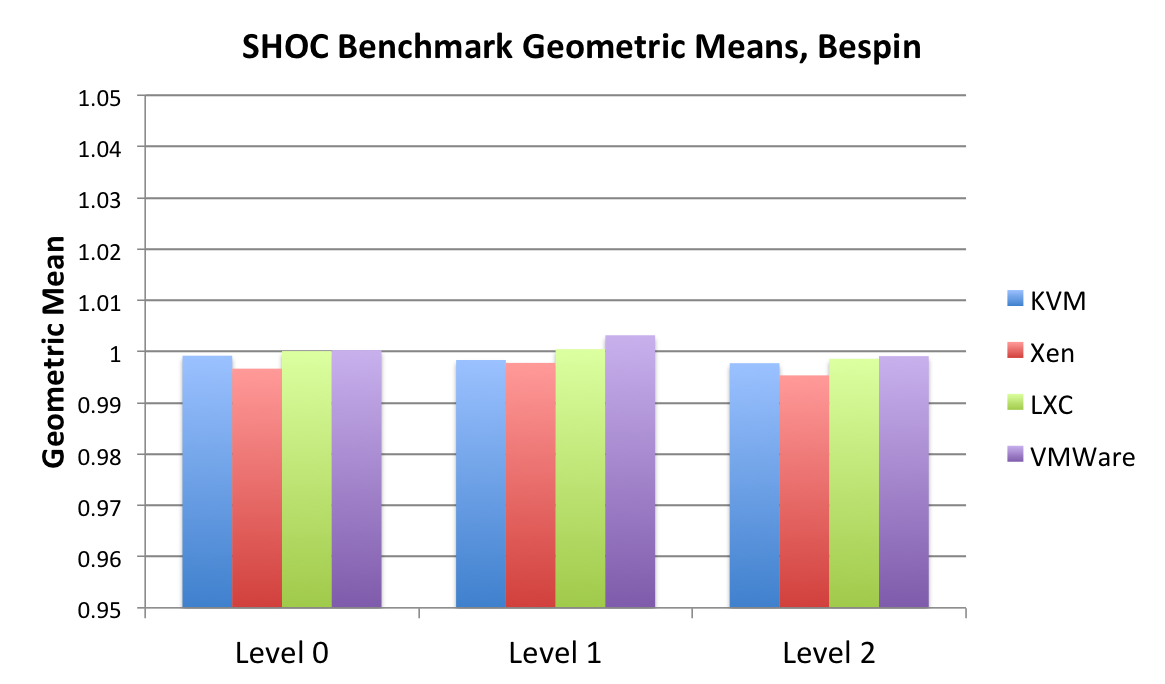
\includegraphics[width=3.25in]{figures/SHOC_means}}
%\caption{SHOC Levels 0-2 geometric means, Bespin hardware.}
%\label{SUMMARY}
%\end{figure}


In Tables~\ref{K20MEANS} and \ref{C2075MEANS}, we provide geometric means for each SHOC level across each
hypervisor and system.  We also include the maximum
overhead for each hypervisor at each level to facilitate comparison across
hypervisors and systems.  Finally, we provide a comparable breakdown of only the
PCIe SHOC benchmarks, based on the intuition that PCIe-specific benchmarks will
likely result in higher overhead.  

At a high level, we immediately notice that in the cases of KVM and LXC, both
perform very near native across both the Bespin and Delta platforms.  On
average, these systems are almost indistinguishable from their non-virtualized
base systems.  So much so, that experimental noise occasionally boosts
performance slightly above their base systems.  

This is in sharp contrast to the Xen and VMWare hypervisors, which perform well
on the Bespin system, but poorly on the Delta system in some cases.  This is
particularly evident when looking at the maximum overheads for Xen and VMWare
across both systems.  In this case, we see that on the Bespin system, Xen's
maximum overhead of 3.34\% is dwarfed by Delta's maximum Xen overhead of 24.0\%.
VMWare exhibits similar characteristics, resulting in a maximum overhead of
1.9\% in the case of the Bespin system, and a surprising 36.6\% in the case of
the Delta system.  We provide a more in-depth discussion of these overheads
below.


\FIGURE{!htb}
  {images/SHOC_L1}
  {1.0}
  {SHOC Levels 0 and 1 relative performance on Bespin system.  Results show benchmarks over or
under-performing by 0.5\% or greater.  Higher is better.}
  {F:SHOC_l1} 

\FIGURE{!htb}
  {images/SHOC_L1-2}
  {1.0}
  {SHOC Levels 1 and 2 relative performance on Bespin system.  Results show benchmarks over or
under-performing by 0.5\% or greater.  Higher is better.}
  {F:SHOC_l1-2} 

\FIGURE{!htb}
  {images/delta-shoc-l0l1}
  {1.0}
  {SHOC Levels 0 and 1 relative performance on Delta system.  Benchmarks
shown are the same as Bespin's.  Higher is better.}
  {F:delta-SHOC_l1} 

\FIGURE{!htb}
  {images/delta-shoc-l1l2}
  {1.0}
  {SHOC Levels 1 and 2 relative performance. Benchmarks shown are the same as
Bespin's.   Higher is better.}
  {F:delta-SHOC_l1-2} 



%\begin{figure}[ht!]
%\centering
%\fbox{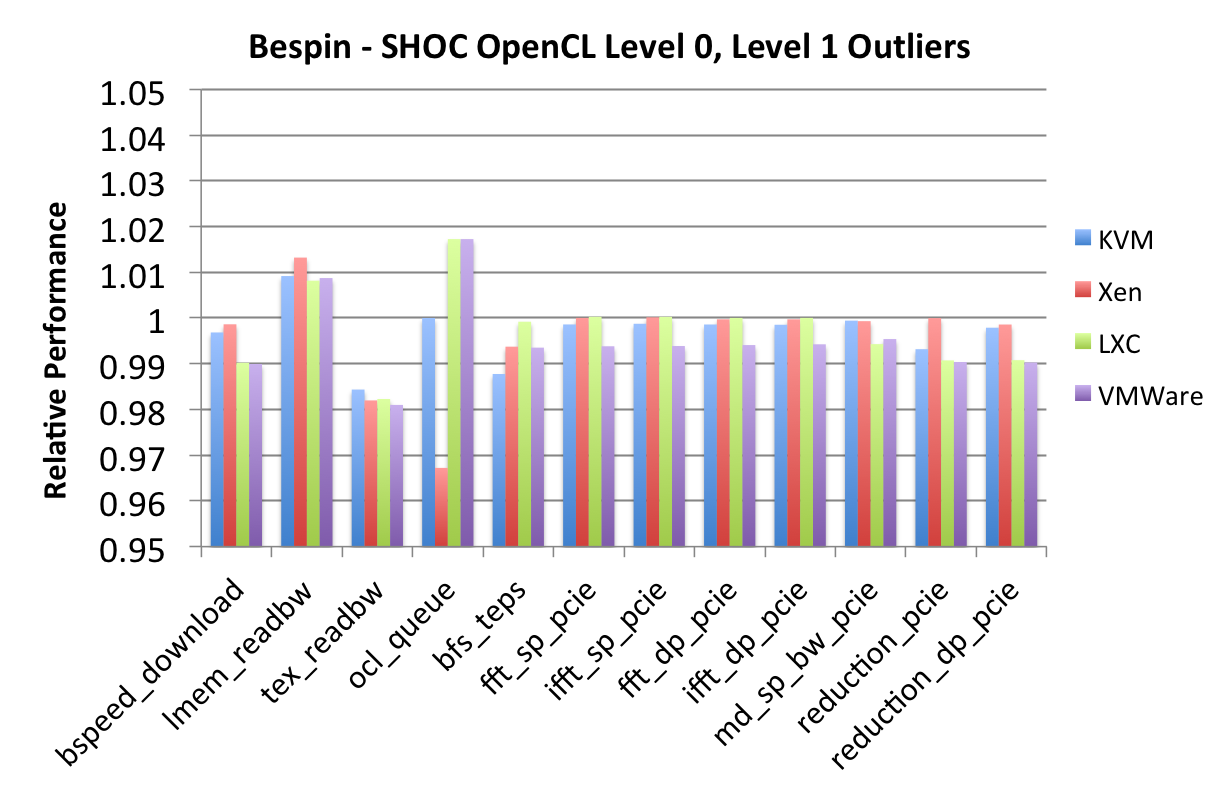
\includegraphics[width=3.25in]{figures/SHOC_L1}}
%\caption{SHOC Levels 0 and 1 relative performance on Bespin system.  Results show benchmarks over or
%under-performing by 0.5\% or greater.  Higher is better.}
%\label{SHOC_l1}
%\end{figure}

%\begin{figure}[ht!]
%\centering
%\fbox{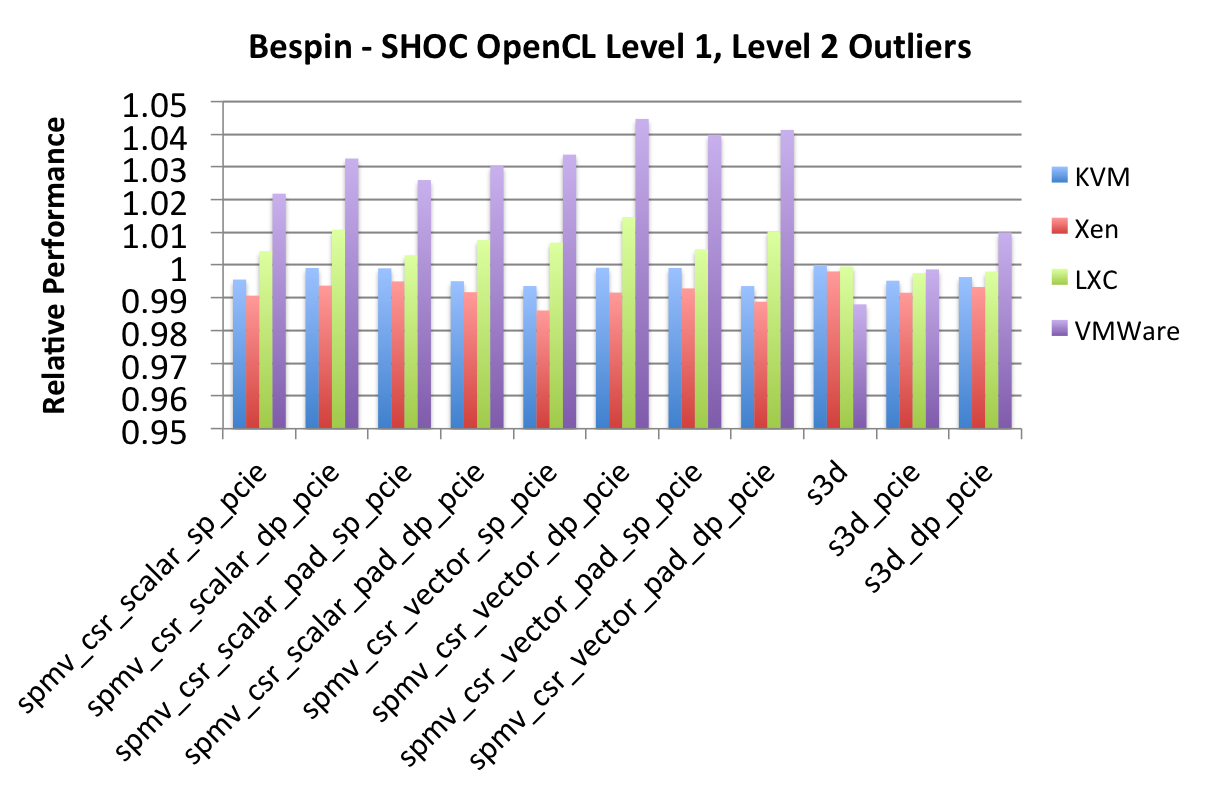
\includegraphics[width=3.25in]{figures/SHOC_L1-2}}
%\caption{SHOC Levels 1 and 2 relative performance on Bespin system.  Results show benchmarks over or
%under-performing by 0.5\% or greater.  Higher is better.}
%\label{SHOC_l1-2}
%\end{figure}

%\begin{figure}[ht!]
%\centering
%\fbox{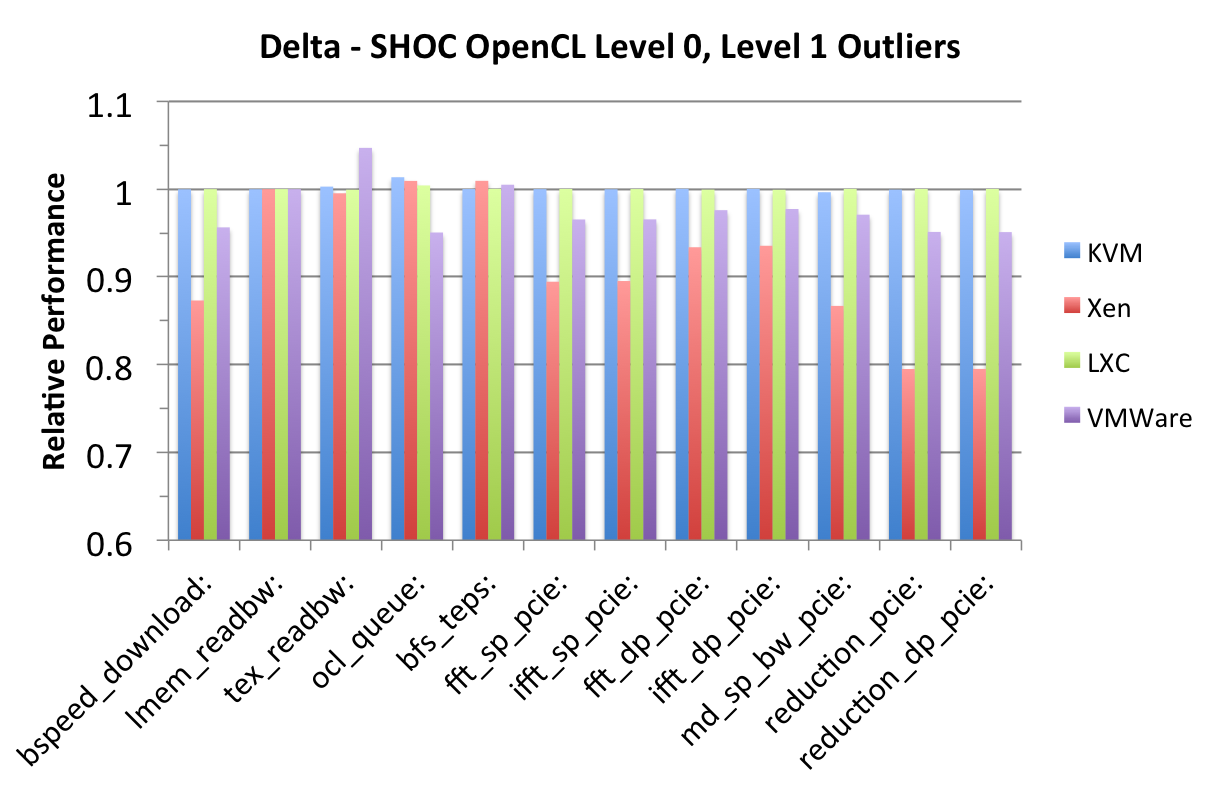
\includegraphics[width=3.25in]{figures/delta-shoc-l0l1.png}}
%\caption{SHOC Levels 0 and 1 relative performance on Delta system.  Benchmarks
%shown are the same as Bespin's.  Higher is better.}
%\label{delta-SHOC_l1}
%\end{figure}

%\begin{figure}[ht!]
%\centering
%\fbox{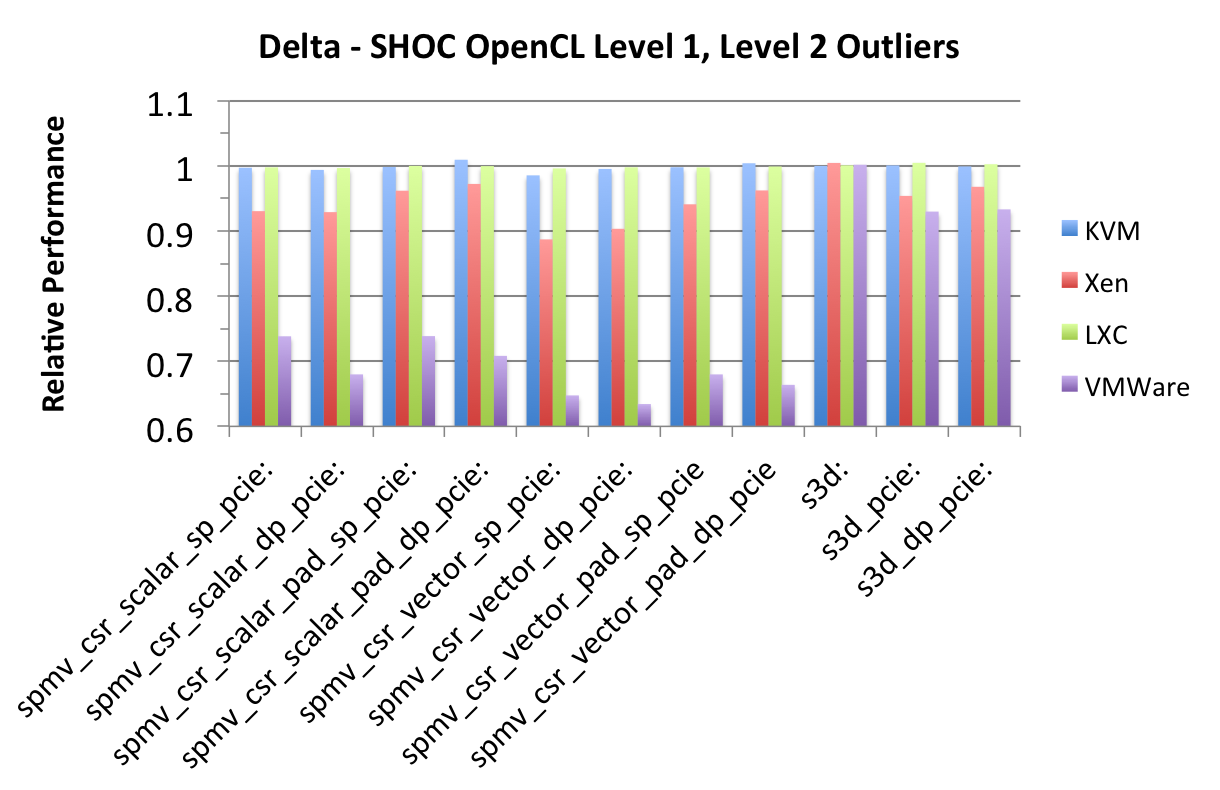
\includegraphics[width=3.25in]{figures/delta-shoc-l1l2.png}}
%\caption{SHOC Levels 1 and 2 relative performance. Benchmarks shown are the same as
%Bespin's.   Higher is better.}
%\label{delta-SHOC_l1-2}
%\end{figure}

%The Bespin
%system, based on a Sandy Bridge CPU with Kepler GPU, averages  99\% efficiency across
%all 4 hypervisors.  Even when considering only the PCIe portion of the SHOC
%benchmarks, virtualization efficiency averages greater than 99\%.   In addition
%to the means, Table~\ref{MEANS} also includes maximum overheads for each SHOC
%level, expressed as a percentage.  In this case we begin to see some slight
%overhead - a maximum of 3.3\% overhead for Xen Level 0 benchmarks, but often
%within 1\% even in the case of the maximum overhead.  

%This contrasts starkly with the Delta system, a Westmere-based Fermi platform,
%which sees overheads as high as 36\% in some cases.  Consequently, the means are
%lowered, particularly in the case of Xen and VMWare for the PCIe-only portion of
%Table~\ref{MEANS}.  Still, KVM and LXC perform very near-native, and under some
%circumstances outpeform the base system.  

%In Figures~\ref{SHOC_l1} and~\ref{SHOC_l1-2} we show the SHOC outlier results
%for the Bespin system.  In Figures~\ref{delta-SHOC_l1} and~\ref{delta-SHOC_l1-2}
%we show the same benchmarks for the Delta system.  We begin the discussion with
%the Bespin system, Figures~\ref{SHOC_l1} and~\ref{SHOC_l1-2}.

Of the Level 0 benchmarks, only four exhibited notable
overhead in the case of the Bespin system: bspeed\_download, lmem\_readbw, tex\_readbw, and ocl\_queue.  These are
shown in Figure~\ref{F:SHOC_l1}.  These benchmarks represent device-level
characteristics, including host-to-device bandwidth, onboard memory reading, and OpenCL
kernel queue delay.  Of the four, only bspeed\_download incurs a statistically
significant overhead.  The remainder perform within one standard deviation of
the base, despite an overhead of greater than 0.5\%.  

bspeed\_download is representative of the most likely source of virtualization overhead, data
movement across the PCI-Express bus.  The PCIe lies at the boundary of
the virtual machine and the physical GPU, and requires interrupt remapping,
IOMMU interaction, etc. in order to enable GPU passthrough into the virtual
machine.  Despite this, in Figure~\ref{F:SHOC_l1} we see a maximum of 1\% overhead
for bspeed\_download in
VMWare, and less than 0.5\% overhead for both KVM and Xen.

The remainder of Figure~\ref{F:SHOC_l1} includes a series of SHOC's Level 1
benchmarks, representing computational kernels.  This includes BFS, FFT, molecular dynamics,
and reduction kernels.  Notably, nearly all of the benchmarks exhibiting
overhead are the PCIe portion of SHOC's benchmarks. This is unsurprising, since
the Level 0 benchmarks suggest PCIe bandwidth as the major source overhead.
Still, results remain consistent with the bspeed\_download overhead observed in
the Level 0 benchmarks, further suggesting that host/device data movement
is the major source of overhead.

In Figure~\ref{F:SHOC_l1-2} we present the remaining SHOC Level 1 results as well
as the SHOC Level 2 results (S3D).  In these results we begin to see an interesting trend,
namely that VMWare consistently outperforms the base system in the Spmv and S3D
microbenchmarks on the Bespin system.  We believe this to be a performance
regression in CentOS 6.4, rather than a unique improvement due to the VMWare ESXi
hypervisor.  When running the benchmarks on a non-virtualized Bespin system with
Arch Linux, the VMWare ESXi performance gains were erased.  An interesting
finding of this was that Spmv was unique in this way - no other benchmarks were
affected by this performance issue.

%We discuss this is more detail in
%Section~\ref{OVERHEADS}.

%We believe this to be a performance regression in
%CentOS 6.4 rather than a unique improvement from VMWare. Executing these
%benchmarks on a non-virtualized Arch Linux system erases VMWare's performance
%gains, suggesting that virtualization, VMWare's Superpages, etc. are not the
%source of the performance improvement.  Nevertheless, we continue to probe the
%performance boost further.

%An interesting characteristic of these benchmarks are that they represent the
%least compute-intensive benchmarks of the entire SHOC suite.  The Spmv
%PCIe benchmarks, for example, perform at less than 1 Gflop/s on both the base
%system as well as the virtual machines.  Because VMWare is the only hypervisor
%to exhibit these characteristics, and because it's closed source, we have
%limited visibility into the low-level performance characteristics.  However, we
%speculate that this may be due to VMWare's very small footprint without even a
%management virtual machine, leaving more resources available to the guest.   

Turning to the Delta system, in Figures~\ref{F:delta-SHOC_l1}
and~\ref{delta-SHOC_l1-2}, we show the same benchmarks for the Delta system as
was shown in Figures~\ref{F:SHOC_l1} and~\ref{F:SHOC_l1-2}.  Again, we find that the
same benchmarks are responsible for most of the overhead on the Delta system.  This is
unsurprising, since PCIe was shown to be the source of the bulk of the overhead.
A major difference in the case of the Delta system, however, is the amount of
overhead.  While the Bespin system saw overheads of approximately 1\%, Delta's overhead
routinely jumps above 35\%, especially in the case of the Spmv benchmark for
VMWare.  

On further examination, we determined that Xen was unable to activate
IOMMU large page tables on the Delta system.  KVM successfully allocated 4k, 2M,
and 1G page table sizes, while Xen was limited to size 4k page tables.  The
Bespin system was able to take advantage of 4k, 2M, and 1G page sizes on both
KVM and Xen.  It appears that this issue is correctable and does not represent a
fundamental limitation to the Xen hypervisor on the Nehalem/Westmere
microarchitecture.  While as a closed source product,  we have limited insight
into VMWare ESXi, we speculate that VMWare may be experiencing a similar issue
on the Delta system and not on our Bespin system.

%In Section~\ref{OVERHEADS}, we provide further context for this high

%overhead, but in short, we do not believe this overhead to be a fundamental
%limitation of the Sandy Bridge architecture.  Rather, at least in Xen's case, it
%appears to be a bug in the handling of IOMMU page table sizes.

In light of this, we broadly find that virtualization overhead across
hypervisors and architectures is minimal.  Questions remain as to the source of the
exceptionally high overhead in the case of Xen and VMWare on the Delta
system, but because KVM shows no evidence of this overhead, we believe the
Westmere/Fermi architecture to be suitable for VGA passthrough in a cloud
environment.  In the case of the Bespin system, it is clear that VGA passthrough can be
achieved across hypervisors with virtually no overhead.  

A surprising finding is that LXC showed little performance advantage over KVM,
Xen, and VWMare.  While we expected near-native performance from LXC we did not expect the
hardware-assisted hypervisors to achieve such high performance.  Still, LXC carries some
advantages.  In general, its maximum overheads are comparable to or less than KVM, Xen, and
VMWare, especially in the case of the Delta system.   

%Broadly, we find that each hypervisor performs near-native even through the
%Level 1 and Level 2 benchmarks.  This is especially true for the Bespin system.
%From Table~\ref{MEANS} we can see that
%KVM and Xen average both achieve greater than 99\% of the base system's
%performance.
%LXC and VMWare both perform nearly identically to the base system, with
%VMWare's results being boosted by the surprising improvement shown in
%Figure~\ref{SHOC_l1-2}.  

%The Delta system shows rather inconsistent behavior.  KVM performs
%well and is nearly identical to its base system.  Xen and VMWare perform well on
%average, but show overheads greater than 20\% under some circumstances,
%particularly the PCIe experiments.  All of
%this suggests that virtualization performance and IOMMU support has improved
%between the Westmere/Nahalem microarchitectures and the Sandy Bridge
%microarchitectures.  It is also notable that KVM performance remains consistent
%between processor generations.  This is encouraging for those who may be
%interested in supporting GPU passthrough in prior-generation hardware.  

%In both systems, we find the LXC results unsurprising, given that it shares a kernel with the
%base system and avoids the overhead of traditional hardware virtualization.
%Still, we find the results of the three remaining hypervisors encouraging for the widespread use of GPUs in the cloud.
%Not only can GPUs be used within a variety of hypervisors, but the performance
%overhead for their use is minimal.  

%\begin{table*}
%\small
%\renewcommand{\arraystretch}{1.3}
%\caption{SHOC level 0 geometric means and max overhead}
%\label{shoc_l0}
%\centering
%\begin{tabular}{|l||l||l|l|}
%\hline
%System & Hypervisor & Max Overhead & Geo. Mean \\ \hline
%Bespin & KVM & 1.57\% & 0.999 \\ \hline
%Bespin & Xen & 3.39\% & 0.997 \\ \hline
%Bespin & LXC & 1.77\% & 1.00 \\ \hline
%Bespin & VMWare & 1.90\% & 1.00 \\ \hline
%\end{tabular}
%\end{table*}


%In Table~\ref{shoc_l1} and Figures~\ref{SHOC_l1}-~\ref{SHOC_l1-2} we provide
%the SHOC Level 1 and Level 2 results.  Because space does not allow us to reproduce each
%benchmark result, we provide summary data in Table~\ref{shoc_l1}, and
%in Figures~\ref{SHOC_l1} and~\ref{SHOC_l1-2}, we show all benchmarks whose
%performance differed by 1\% or more from the base CentOS system.  

%Again, each hypervisor performs within 1\% of the native CentOS system.
%However, as shown in Figures~\ref{SHOC_l1} and~\ref{SHOC_l1-2}, there are
%occasions in which the virtualized guest outperforms the host by as much as
%4.3\%.  The vast majority of the benchmarks that either outperformed or
%underperformed with respect to the base system, are the PCIe variants of the
%SHOC suite.  This is perhaps unsurprising, since the GPU itself isn't
%virtualized, and we would expect that PCIe transactions would be the source of
%the bulk of the overhead.  More surprising, however, is that VMWare ESXi is able
%to consistently outperform the host system for the SPMV (sparse matrix dense
%vector multiplication) benchmarks.  VMWare is the most extreme example, but Xen
%too occasionally outperforms the host.

%(XXX why?  Not sure, but one possibility, the SPMV kernels are comparably low performing, like 0.918 GFLOP/s
%whereas the SGEMM kernels are much higher, 230 GFLOP/s - 550 GFLOP/s even under
%the PCIe test.)



%\begin{table}
%\small
%\renewcommand{\arraystretch}{1.3}
%\caption{SHOC levels 1 and 2 geometric means and max overhead.  Level 2 means
%are in parentheses.}
%\label{shoc_l1}
%\centering
%\begin{tabular}{|l||l||l|l|}
%\hline
%System & Hypervisor & Max Overhead & Geo. Mean \\ \hline
%Bespin & KVM & 1.75\% &  0.999 (0.999) \\ \hline
%Bespin & Xen & 6.15\% &  0.990 (0.982) \\ \hline
%Bespin & LXC & 0.72\% &  1.00 (1.00) \\ \hline
%bespin & VMWare & 0.63\% &  1.00 (1.00) \\ \hline
%\end{tabular}
%\end{table}

\subsection{GPU-LIBSVM Performance}



\FIGURE{!htb}
  {images/libSVM}
  {1.0}
  {GPU-LIBSVM relative performance on Bespin system.  Higher is better.}
  {F:LIBSVM} 

\FIGURE{!htb}
  {images/libSVM}
  {1.0}
  {GPU-LIBSVM relative performance on Delta showing improved performance
within virtual environments.  Higher is better.}
  {F:delta-LIBSVM} 



%\begin{figure}[ht!]
%\centering
%\fbox{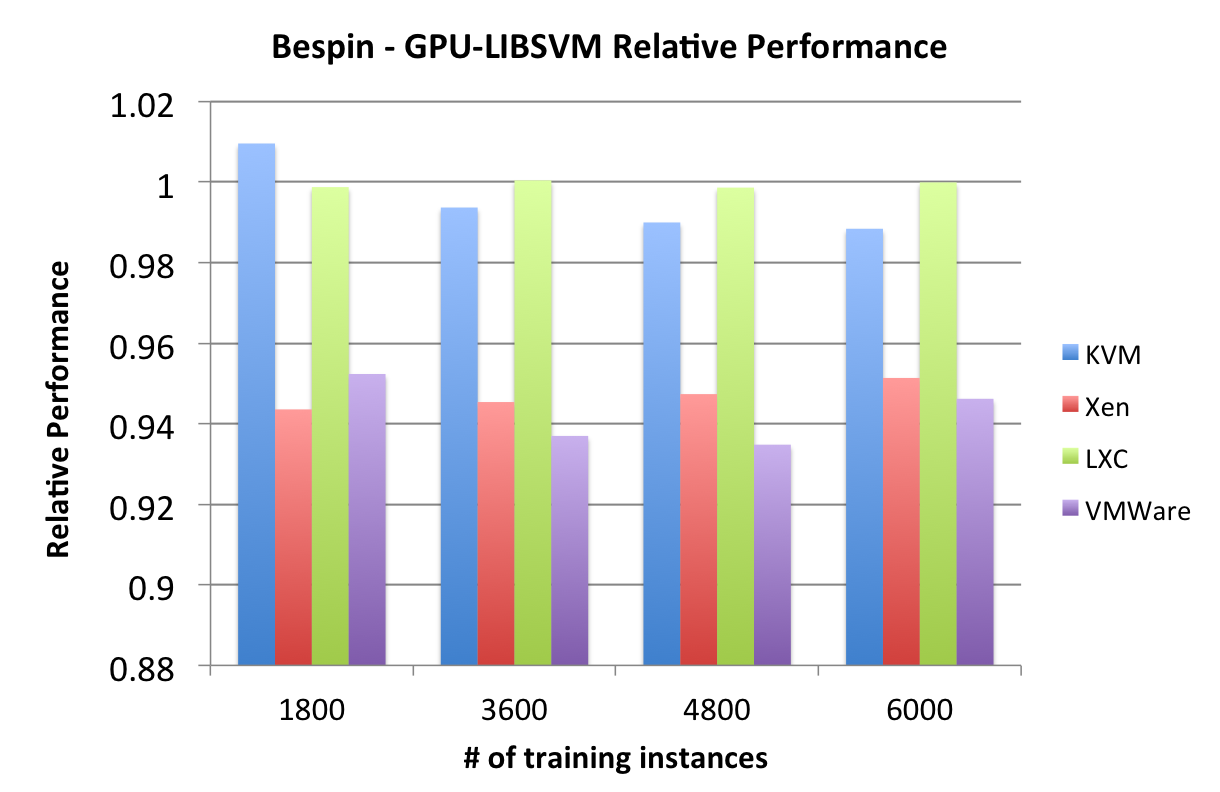
\includegraphics[width=3.25in]{figures/libSVM}}
%\caption{GPU-LIBSVM relative performance on Bespin system.  Higher is better.}
%\label{LIBSVM}
%\end{figure}

%\begin{figure}[ht!]
%\centering
%\fbox{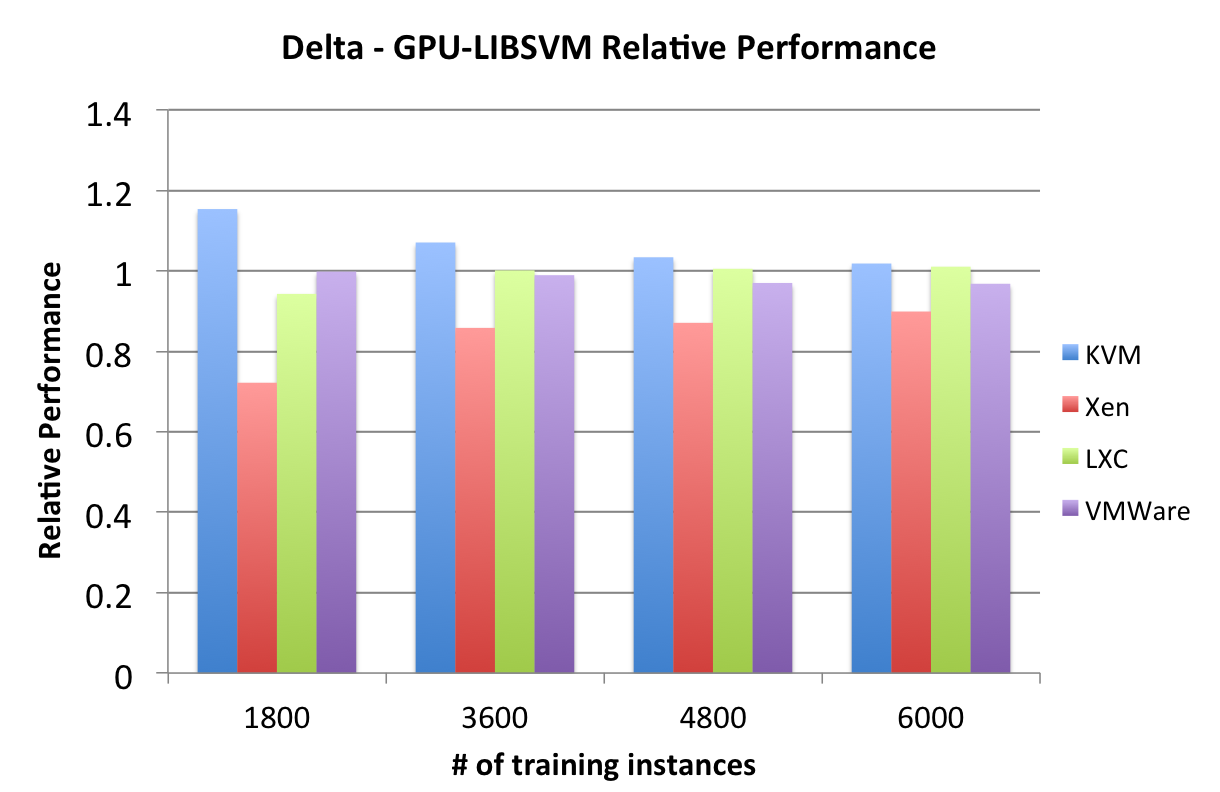
\includegraphics[width=3.25in]{figures/delta-libsvm-rel.png}}
%\caption{GPU-LIBSVM relative performance on Delta showing improved performance
%within virtual environments.  Higher is better.}
%\label{delta-LIBSVM}
%\end{figure}

In Figures~\ref{F:LIBSVM} and~\ref{F:delta-LIBSVM}, we display our GPU-LIBSVM performance results for the
Bespin (K20m) and Delta (C2075) systems. Using the NIPS 2003 gisette data set, we show the
performance across 4 problems sizes, ranging from 1800 to 6000 training
instances. The NIPS 2003 gisette dataset is a standard dataset that was used as a part of
the NIPS 2003 feature selection challenge. 

KVM again performs well across both the Delta and Bespin systems.  In the case
of the Delta system, in fact, KVM, significantly outperforms the base
system.  We determined this to be caused by KVM's support for transparent
hugepages.  When sufficient memory is available, transparent hugepages may be
used to back the entirety of the guest VM's memory.  Hugepages have previously
been shown to improve TLB performance for KVM guests, and have been shown to
occasionally boost the performance of a KVM guests beyond its
host~\cite{Arcangeli:2010}.  After disabling hugepages on the KVM host for the
Delta system, performance dropped to 80--87\% of the base system, suggesting that
memory optimizations such as transparent hugepages can substantially improve the
performance of virtualized guests under some circumstances.  LXC and VMWare
perform close to the base system, while Xen achieves between 72--90\% of the
base system's performance.  We speculate that this may be related to Xen's
inability to enabled page sizes larger than 4k.

%Another unusual characteristic of the
%GPU-LIBSVM benchmarks is that LXC performs unusually poorly for small problem
%sizes on the Delta system.  This effect is not apparent on the Bespin system,
%and its cause on the Delta system is under investigation. Xen performs comparably across both systems, ranging from 96 - 99\% efficiency
%in the case of Bespin, and maintaining 96\% efficiency on the Delta system.  

%GPU-LIBSVM is unique among our studied benchmarks,
%  in that the virtualization layer itself improves
%performance in the case of KVM and VMWare.  We explore this in more detail in
%Section~\ref{OVERHEADS}.


%This is accomplished through the use of
%transparent hugepages (THP), which are known to improve TLB performance for KVM
%guests~\cite{LINUXCONF}.  In some cases, this has resulted in improved performance over the base
%system~\cite{LINUXCONF}.  VMWare ESXi supports a related technology, Superpages;
%and as we show in Figure~\ref{delta-LIBSVM}, VMWare is also capable of
%ourperforming the base system, especially for small problem sizes.  

%The degree of performance boost depends largely on the problem size and system
%architecture.  In the case of our Bespin system, hugepages result in only a
%slight performance boost, and only for the smallest problem size.  In the case
%of the Delta system, however, performance boosts of nearly 40\% for KVM, and
%20\% for VMWare are possible.  While the effect of hugepages and superpages
%decreases for increasing problem sizes, there is still a noticeable impact on
%Delta for hugepages at all problem sizes.  When disabling transparent hugepages;
%however, performance returns to XXXSOMETHINGXXX, comparable with the host.

%For the smallest problem size of 1800 (XXXSOMETHINGSXXX), the use of THP boosts
%performance slightly higher than the base system.  The improvement disappears
%both as problem sizes increase, and when THP are disabled.  In
%Figure~\ref{LIBSVM}, we provide performance both for hugepages enabled and
%disabled for the KVM hypervisor.      

\subsection{LAMMPS Performance}

\FIGURE{!htb}
  {images/rhodo}
  {1.0}
  {LAMMPS Rhodopsin benchmark relative performance for Bespin system.  Higher is better.}
  {F:RHODO} 


\FIGURE{!htb}
  {images/delta-lammps-rhodo}
  {1.0}
  {LAMMPS Rhodopsin benchmark relative performance for Delta system.  Higher is better.}
  {F:delta-RHODO} 


%\begin{figure}[ht!]
%\centering
%\fbox{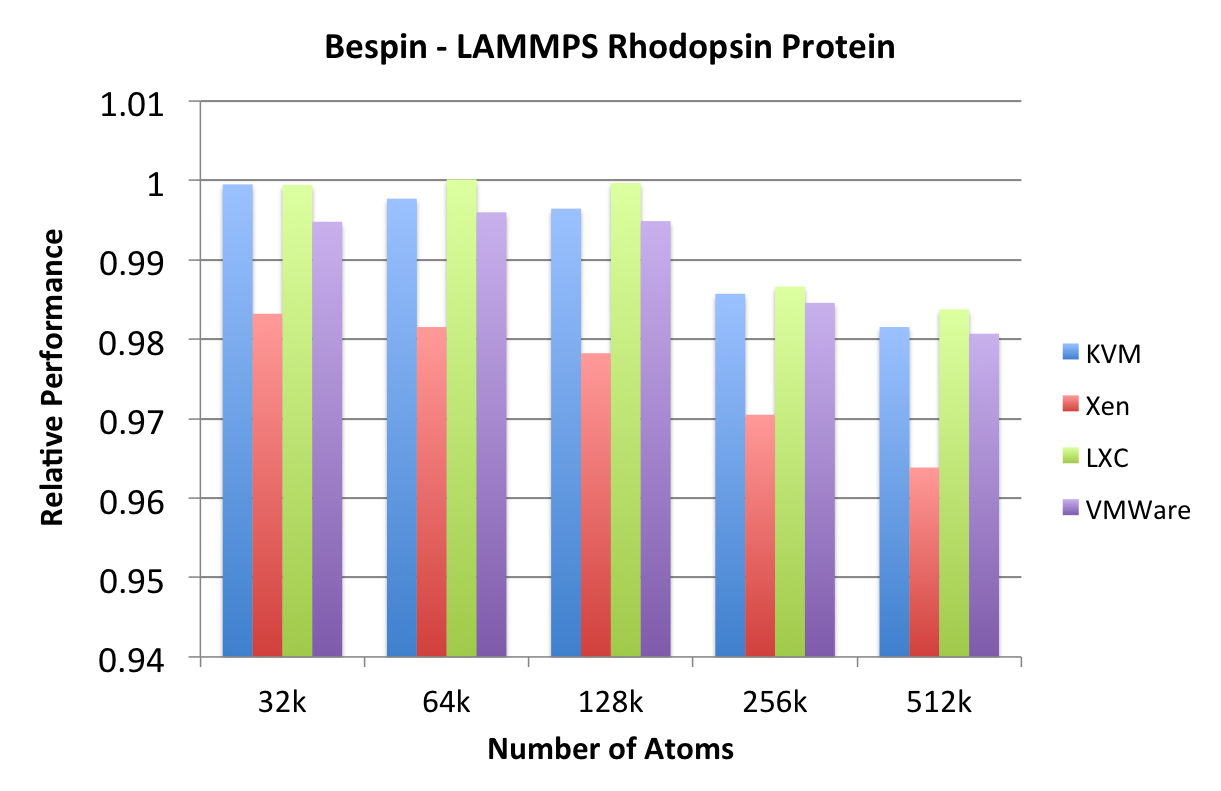
\includegraphics[width=3.25in]{figures/rhodo}}
%\caption{LAMMPS Rhodopsin benchmark relative performance for Bespin system.  Higher is better.}
%\label{RHODO}
%\end{figure}


%\begin{figure}[ht!]
%\centering
%\fbox{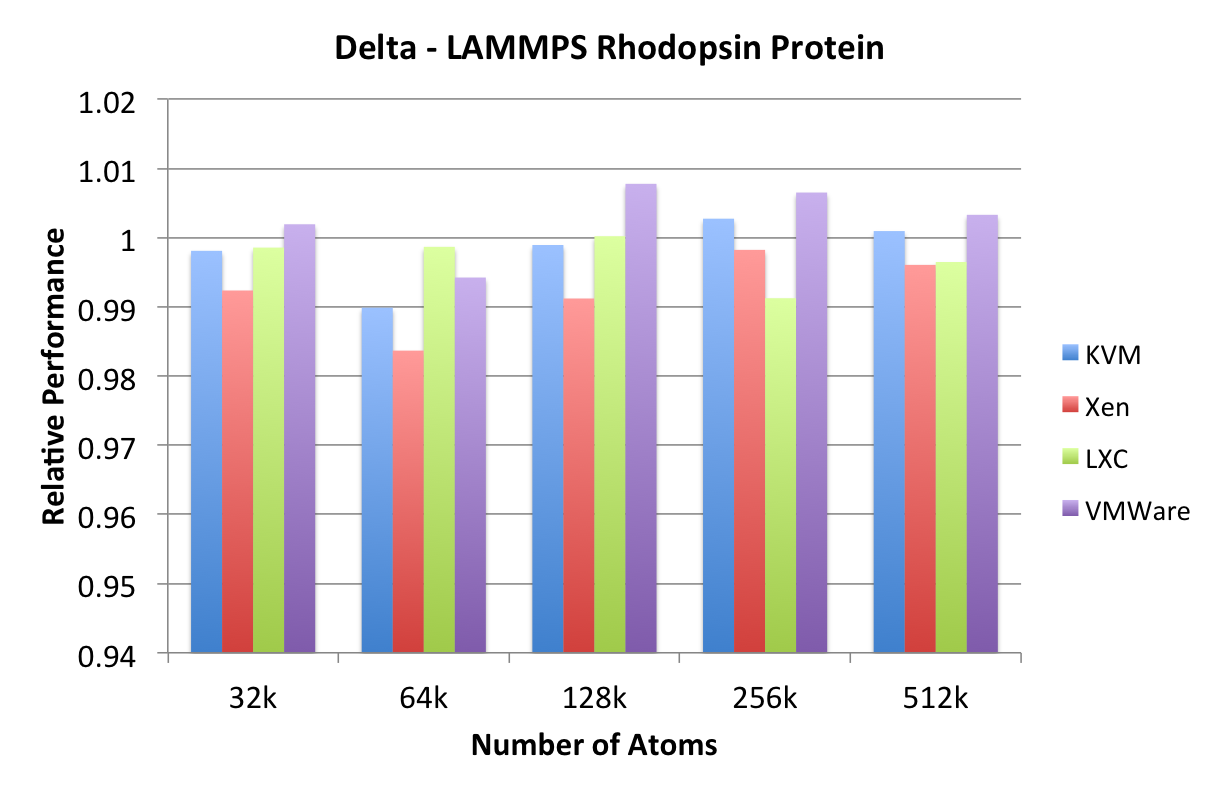
\includegraphics[width=3.25in]{figures/delta-lammps-rhodo}}
%\caption{LAMMPS Rhodopsin benchmark relative performance for Delta system.  Higher is better.}
%\label{delta-RHODO}
%\end{figure}

In Figures~\ref{F:RHODO} and~\ref{F:delta-RHODO}, we show the LAMMPS Rhodopsin protein simulation results.
LAMMPS is unique among our benchmarks, in that it exercises both the GPU and
multiple CPU cores.  In keeping with the LAMMPS benchmarking methodology, we
execute the benchmark using 1 GPU and 1--8 CPU cores
on the Bespin system,
selecting the highest performing configuration.  In the case of the Delta
system, we execute the benchmark on 1--6 cores and 1 GPU, selecting the highest
performing configuration.

Overall, LAMMPS performs well across both hypervisors and systems.
Surprisingly, LAMMPS showed better efficiency on the Delta system than the
Bespin system, achieving greater than 98\% efficiency across the board, while
Xen on the Bespin system occasionally drops as low as 96.5\% efficiency. 

This performance is encouraging because it suggests that even heterogeneous CPU
+ GPU code is capable of performing well in a virtualized environment.  Unlike
SHOC, GPU-LIBSVM, and LULESH, LAMMPS fully exercises multiple host CPUs,
splitting work between one or more GPUs and one or more CPU cores.  This has the
potential to introduce additional performance overhead, but the results do not
bear this out in the case of LAMMPS.  

%As the problem size (number of atoms) increases, LAMMPS is able to more
%effectively use a greater number of CPU cores.  Between 32k and 128k atoms, 4
%and 6 cores are the highest performing configurations.  This results in greater
%than 99\% efficiency for all but the Xen hypervisor.  

%There is a slight decrease in efficiency at 256k and 512k atom configurations.
%These configurations use all 8 CPU cores available to the VM.  The apparent
%overhead is unrelated to virtualization.  Instead, it is simply due to the host
%system offloading operating system tasks to the 8 additional cores and
%dedicating a full 8 cores to LAMMPS, while the virtual machines' 8 cores
%balanced LAMMPS computation and other operating system-related tasks.  This is
%not an overhead due to virtualization, but rather a resource advantage on the
%part of the host system.  Restricting the base system to 8 cores and 24G RAM,
%resulted in performance comparable to the virtual machines.

\subsection{LULESH Performance}

In Figure~\ref{F:LULESH_bespin} we present our LULESH results for problem sizes
ranging from mesh resolutions of $N=30$ to $N=150$.  LULESH is a highly compute-intensive
simulation, with limited data movement between the host/virtual machine and the
GPU, making it ideal for GPU acceleration. Consequently, we would expect
little overhead due to virtualization. We show LULESH results only on the Bespin
system, because differences in the code bases between the Kepler and Fermi
implementations led to unsound comparisons.

While, overall, we see very little overhead, there is a
slight scaling effect that is most apparent in the case of the Xen hypervisor.
As the mesh resolution ($N^3$) increases from $N=30$ to $N=150$, we see that the Xen
overhead decreases until Xen performs on-par with
KVM, LXC, and VMWare.  


\FIGURE{!htb}
  {images/LULESH_bespin}
  {1.0}
  {LULESH relative performance on Bespin. Higher is better.}
  {F:LULESH_bespin} 

%\begin{figure}[ht!]
%\centering
%\fbox{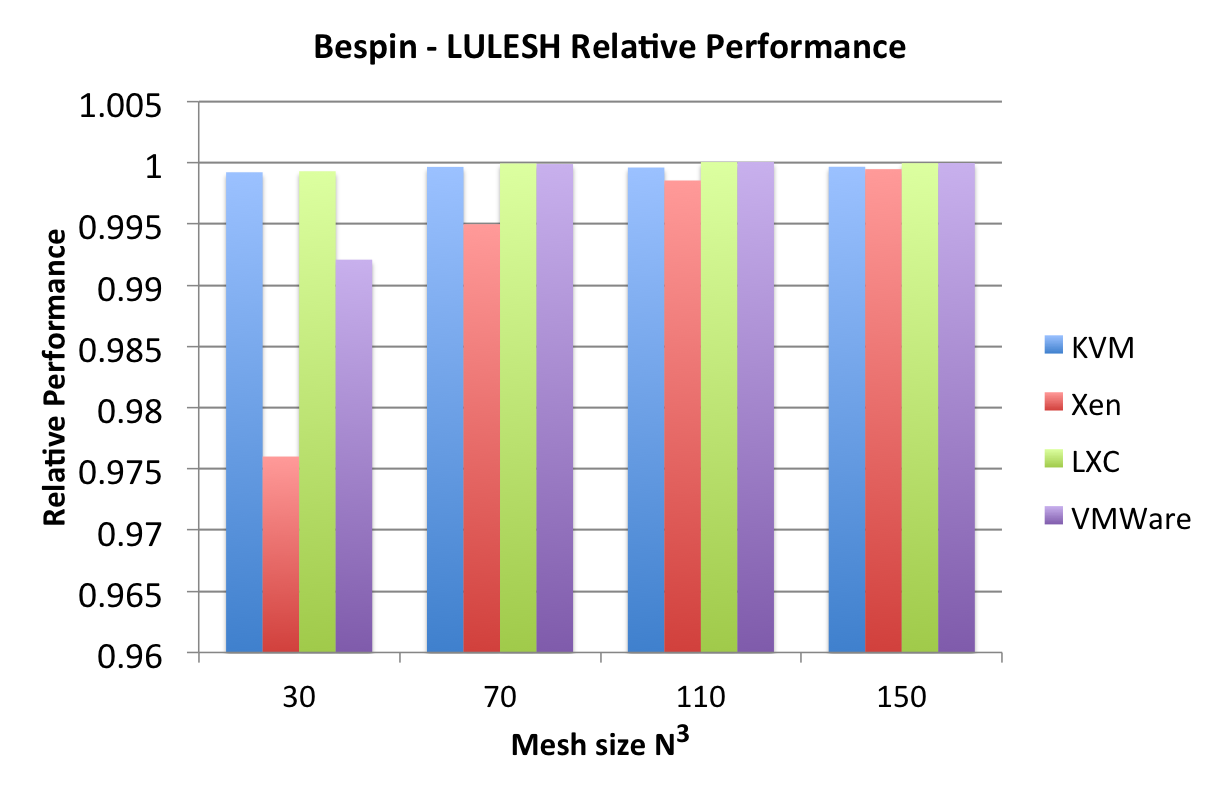
\includegraphics[width=3.25in]{figures/LULESH_bespin}}
%\caption{LULESH relative performance on Bespin. Higher is better.}
%\label{LULESH_bespin}
%\end{figure}


\section{Lessons Learned}\label{LESSONS}
%The primary lesson learned through this experiment is that in the span of a single microarchitectural generation, virtualization
%performance has improved dramatically.  While we've shown that prior processor
%generations at times impose a significant performance penalty, even when paired
%with a non-virtualized GPU, today's processors have reduced that penalty (on
%avereage) to less than 1\%.  

Virtualizing performance-critical workloads has always proven controversial,
whether the workload is CPU-only \cite{Younge2011cloud} or CPU with GPU.  From our Westmere results, we
can see that this criticism is in part legitimate, at times resulting in a performance
penalty of greater than 10\%, especially in the case of the VMWare ESXi and Xen
hypervisors.  We believe much of this to be fixable, especially in the case of
the Xen hypervisor.  

At the same time, however, we have shown that the Sandy Bridge
processor generation has nearly erased those performance overheads, suggesting
that old arguments against virtualization for performance-critical tasks should
be reconsidered.  In light of this, the primary lesson from this study is that VGA-passthrough to
virtual machines is achievable at low overhead, and across a variety of
hypervisors and virtualization platforms.  Virtualization performance remains
inconsistent across hypervisors for the Westmere generation of processors, but
starting with the Sandy Bridge architecture, performance and consistency
increase dramatically.  In the case of the Sandy Bridge architecture, even the lowest performing hypervisor, open source Xen, typically
performs within 95\% of the base case.

This study has also yielded valuable insight into the merits of each hypervisor.
KVM consistently yielded near-native performance across the full range of
benchmarks.  Its support for transparent hugepages resulted in slight
performance boosts over-and-above even the base CentOS system in the case of the
Delta system.  

%This was true
%across both the Delta (C2075) and Bespin (K20) systems, but the effect was much
%greater in the case of the Delta system.  

VMWare's performance proved inconsistent across architectures, performing well
in the case of Bespin, and relatively poorly in the case of the Delta system.
Because hypervisor configurations were identical across systems, we can only speculate that
VMWare's performance is aided by the virtualization improvements offered by the
Sandy Bridge microarchitecture.  

The Xen hypervisor was consistently average across both architectures,
performing neither poorly nor extraordinarily well in any individual benchmark.
Xen and VMWare ESXi are the only two hypervisors from this study that officially support VGA
passthrough.  As a result, PCI passthrough support in both Xen and VMWare is
more robust than KVM.  We expect that this advantage will not last long, as
commercial solutions targeting PCI passthrough in KVM are becoming
common, particularly with regard to SR-IOV and networking adapters.

Linux Containers (LXC), consistently performed closest to the native case.
This, of course, is not surprising given that LXC guests share a
single kernel with their hosts.  This performance comes at the cost of both
flexibility and security, however.  LXC is less flexible than its full
virtualization counterparts, offering
support for only Linux guests.  More importantly, LXC device
passthrough has security implications for multi-GPU systems.  In the case of
a multi-GPU-enabled host with NVIDIA hardware, both GPUs must be passed to the
LXC guest in order to initialize the driver.  This limitation may be addressable
in future revisions to the NVIDIA driver. 


\section{Directions for Future Work}\label{FUTURE}
In this chapter we have characterized the performance of 4 common hypervisors
across two generations of GPUs and two host microarchitectures, and across 3
sets of benchmarks.  We showed the dramatic improvement in virtualization
performance between the Fermi/Westmere and the Kepler/Sandy Bridge system, with
the Sandy Bridge system typically performing within 1\% of the base system.
Finally, this study sought to characterize the GPU and CPU+GPU performance with
carefully tuned hypervisor and guest configurations, especially with respect to
NUMA.  Improvements must be made to today's hypervisors in order
to improve virtual NUMA support. Finally, cloud infrastructure, such as OpenStack, must be capable
of automatically allocating virtual machines in a NUMA-friendly manner in order
to achieve acceptable results at cloud-scale.

%This has implications for virtualized high performance computing in addition to
%the single GPU-enabled nodes shown in this paper.

The next step in this work is to move beyond the single node to show that
clusters of accelerators can be efficiently used with minimal overhead.  This
will require studies in high speed networking, particularly SR-IOV-enabled 
ethernet and Infiniband.  Special attention is needed to ensure that
latencies remain tolerable within virtual environments.  Some studies have begun
to examine these issues~\cite{SRIOVInfiniband}, but open questions remain.


%Virtual NUMA support for the
%hypervisors in this study ranged from non-existent, to commercially supported.






